\documentclass[12pt,a4paper]{article}

% Font and encoding
\usepackage[utf8]{inputenc}
\usepackage[T1]{fontenc}

% Layout
\usepackage[top=1.8cm, bottom=1.8cm, left=2cm, right=2cm]{geometry}
\usepackage{setspace}
\usepackage{indentfirst}

% Graphics
\usepackage{graphicx}
\graphicspath{{../images/}}
\usepackage{caption}
\usepackage{subcaption}

% Math
\usepackage{amsmath}
\usepackage{amssymb}

% Tables
\usepackage{array}
\usepackage{booktabs}
\usepackage{tabularx}

% Hyperlinks
\usepackage[colorlinks=true, linkcolor=blue, citecolor=blue, urlcolor=blue]{hyperref}

% Section spacing
\usepackage[compact]{titlesec}
\titlespacing{\section}{0pt}{4pt}{2pt}
\titlespacing{\subsection}{0pt}{3pt}{1pt}

% Header/footer
\usepackage{fancyhdr}
\setlength{\headheight}{14pt}
\pagestyle{fancy}
\fancyhf{}
\rhead{\small Laporan Eksperimen Operasi Sinyal dan Citra}
\lhead{\small Pengolahan Sinyal Digital}
\rfoot{\thepage}
\renewcommand{\headrulewidth}{0.4pt}

\begin{document}

\begin{titlepage}
\begin{center}
\vspace*{1cm}
\Large\textbf{LAPORAN EKSPERIMEN}\\[0.3cm]
\Large\textbf{OPERASI DASAR PADA SINYAL DAN CITRA}\\[0.6cm]
\normalsize
Mata Kuliah: Pengolahan Sinyal Digital\\[1cm]
\small
\textbf{Identitas Mahasiswa:}\\
Nama: Farrel Ghozy Affifudin\\
NIM: 452024611053\\
Kelas: TI 5 A2\\
Program Studi: Teknik Informatika\\[1cm]
\vfill
\small
\textbf{Program Studi Teknik Informatika}\\
\textbf{Fakultas Sains dan Teknologi}\\
\textbf{Universitas Darussalam Gontor}\\
\today
\end{center}
\end{titlepage}

\singlespacing
\setlength{\parskip}{2pt}
\setlength{\floatsep}{4pt}
\setlength{\textfloatsep}{4pt}
\setlength{\intextsep}{4pt}

% ============================================================
\section{Pendahuluan}
% ============================================================

Pengolahan Sinyal Digital (Digital Signal Processing / DSP) merupakan cabang ilmu yang mempelajari representasi, manipulasi, dan analisis sinyal dalam bentuk diskrit. Operasi dasar seperti penjumlahan, penggeseran, dan amplifikasi menjadi fondasi bagi konsep yang lebih besar seperti superposisi, sistem linier, filtering, hingga augmentasi citra.

Laporan ini menyajikan hasil eksperimen penerapan operasi dasar pada sinyal 1D dan citra 2D menggunakan Python. Eksperimen mencakup pembuatan sinyal diskrit, operasi penjumlahan, penggeseran, amplifikasi, uji sistem linier, serta analisis HOTS (Higher Order Thinking Skills) yang menghubungkan konsep dengan aplikasi nyata.

% ============================================================
\section{Operasi pada Sinyal 1D}
% ============================================================

\subsection{Membuat Sinyal Diskrit}

Dua sinyal diskrit dibuat dalam rentang $n = 0,1,2,\dots,30$:
\begin{align*}
x_1[n] &= \sin(0.5\pi n) \quad \text{(sinusoidal)} \\
x_2[n] &= u[n-5] = \begin{cases}
0, & n < 5 \\
1, & n \geq 5
\end{cases} \quad \text{(unit step)}
\end{align*}

\begin{figure}[h]
\centering
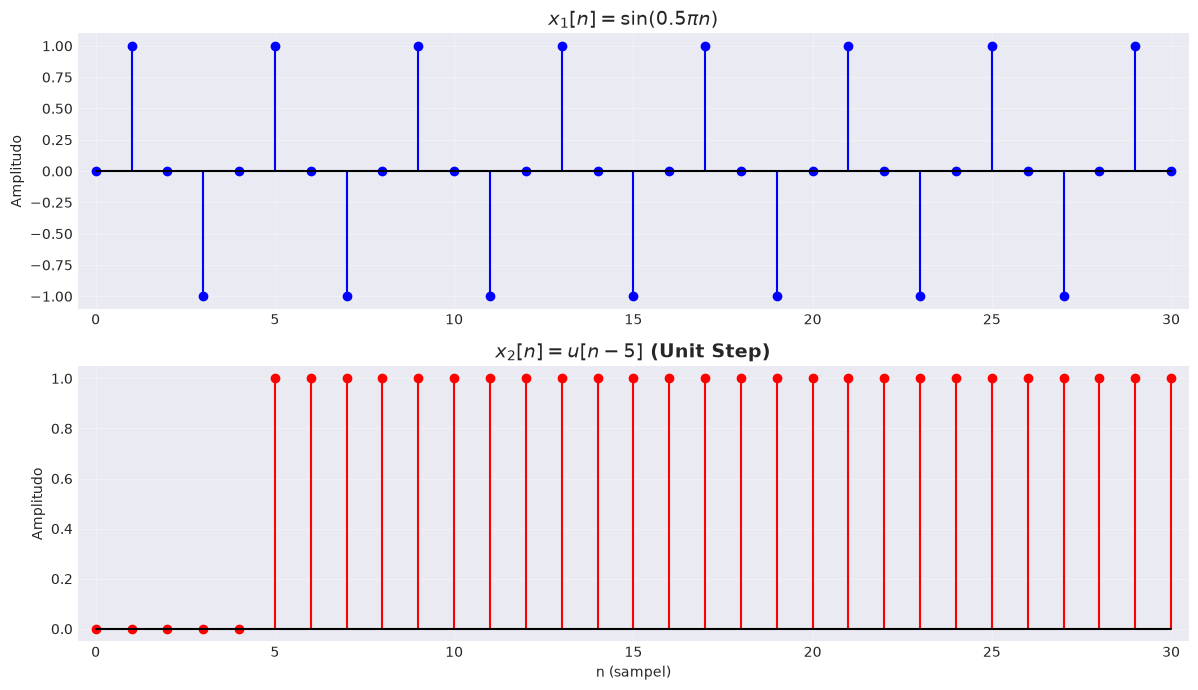
\includegraphics[width=0.65\textwidth]{sinyal_x1_x2.png}
\caption{Sinyal $x_1[n]$ (sinusoidal) dan $x_2[n]$ (unit step).}
\end{figure}

Sinyal $x_1[n]$ bersifat periodik dengan periode $N=4$ dan amplitudo antara $-1$ hingga $1$. Sinyal $x_2[n]$ bersifat aperiodik dengan transisi mendadak dari 0 ke 1 pada $n=5$.

\subsection{Penjumlahan Sinyal}

Operasi penjumlahan $y[n] = x_1[n] + x_2[n]$ menghasilkan superposisi amplitudo. Untuk $n < 5$, $y[n] = x_1[n]$ karena $x_2[n]=0$. Untuk $n \geq 5$, terjadi \textit{DC shift} sebesar +1 sehingga amplitudo maksimum menjadi 2.

\begin{figure}[h]
\centering
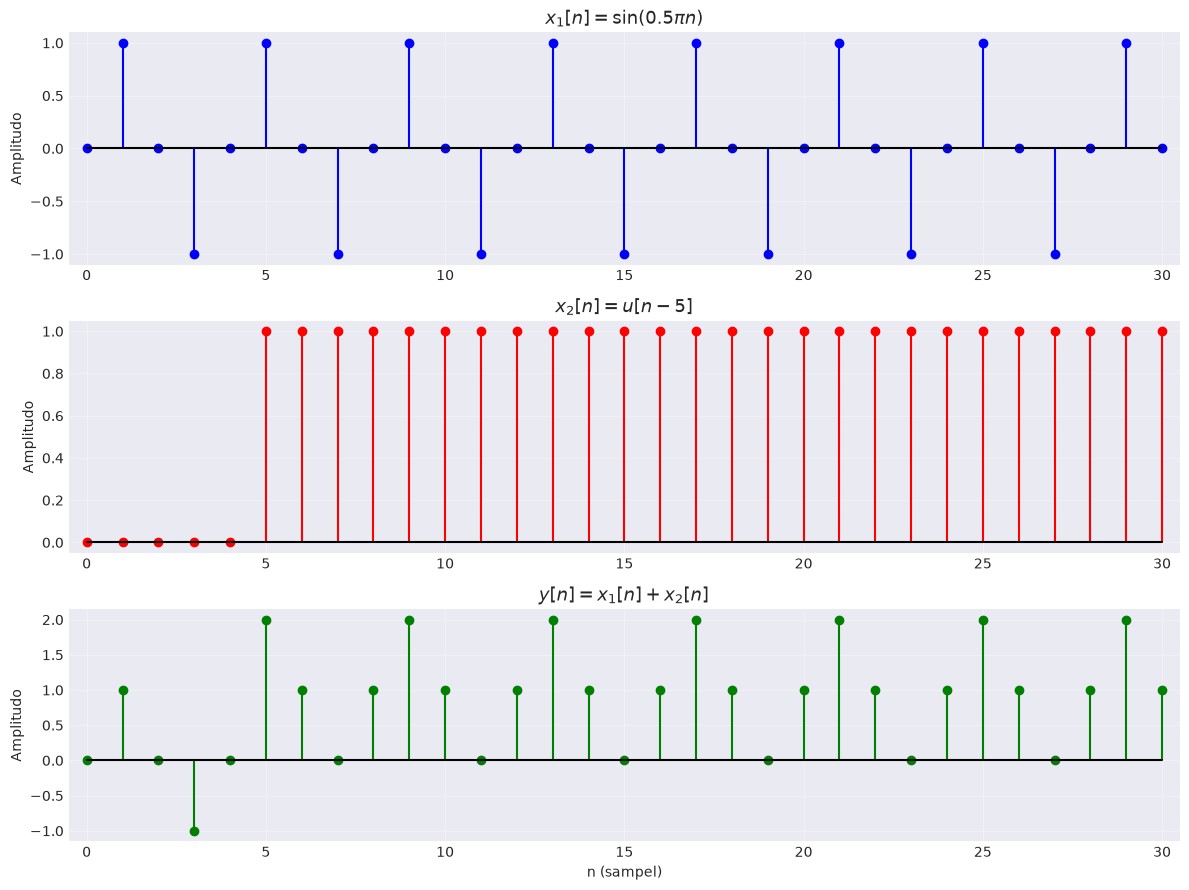
\includegraphics[width=0.6\textwidth]{penjumlahan_sinyal.png}
\caption{Hasil penjumlahan sinyal $y[n] = x_1[n] + x_2[n]$.}
\end{figure}

\textbf{Analisis:} Amplitudo meningkat karena adanya superposisi. Bentuk sinusoidal tetap dominan dengan tambahan DC offset. Aplikasi nyata: \textit{audio mixing}, \textit{sensor fusion}, dan \textit{noise cancellation}.

\subsection{Penggeseran Sinyal}

Penggeseran $y[n] = x[n-k]$ diuji dengan $k = -3$, $0$, dan $4$.

\begin{figure}[h]
\centering
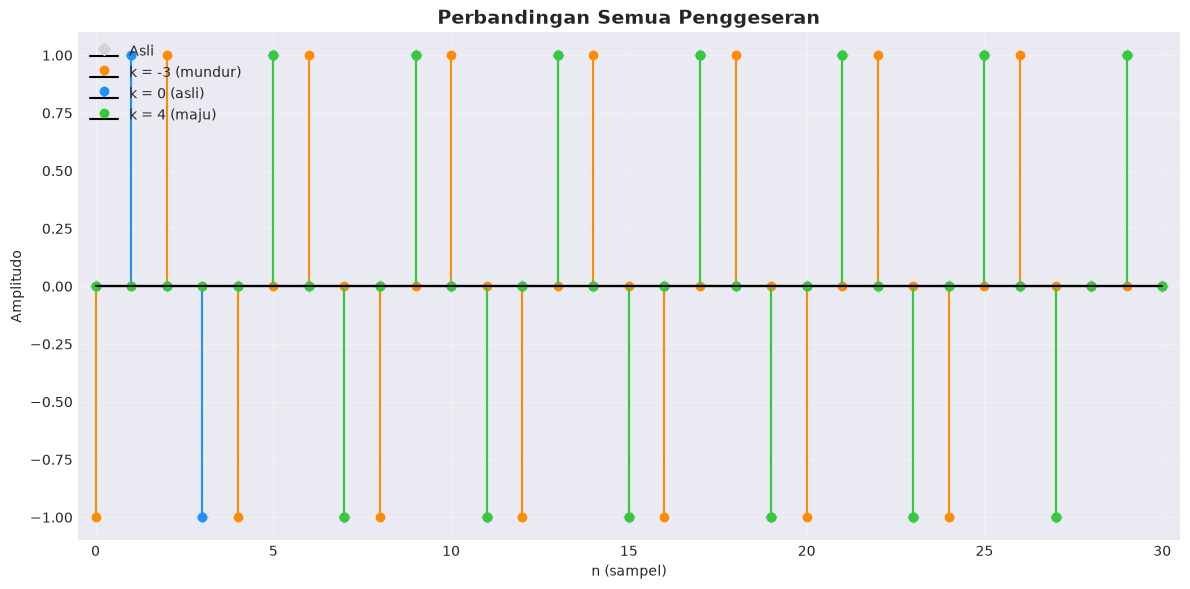
\includegraphics[width=0.6\textwidth]{penggeseran_sinyal_komparasi.png}
\caption{Perbandingan hasil penggeseran sinyal dengan berbagai nilai $k$.}
\end{figure}

$k$ positif menyebabkan \textit{delay} (sinyal bergeser ke kanan), sedangkan $k$ negatif menyebabkan \textit{advance} (sinyal bergeser ke kiri). Pada $k=4$, nilai 4 sampel pertama menjadi 0 (\textit{zero-padding}). Konsep ini digunakan untuk simulasi \textit{delay} pada sistem audio dan \textit{time alignment} dalam komunikasi.

\subsection{Amplifikasi Sinyal}

Amplifikasi $y[n] = \alpha x[n]$ diuji dengan $\alpha = 0.5$, $1$, $2$, dan $-1$.

\begin{figure}[h]
\centering
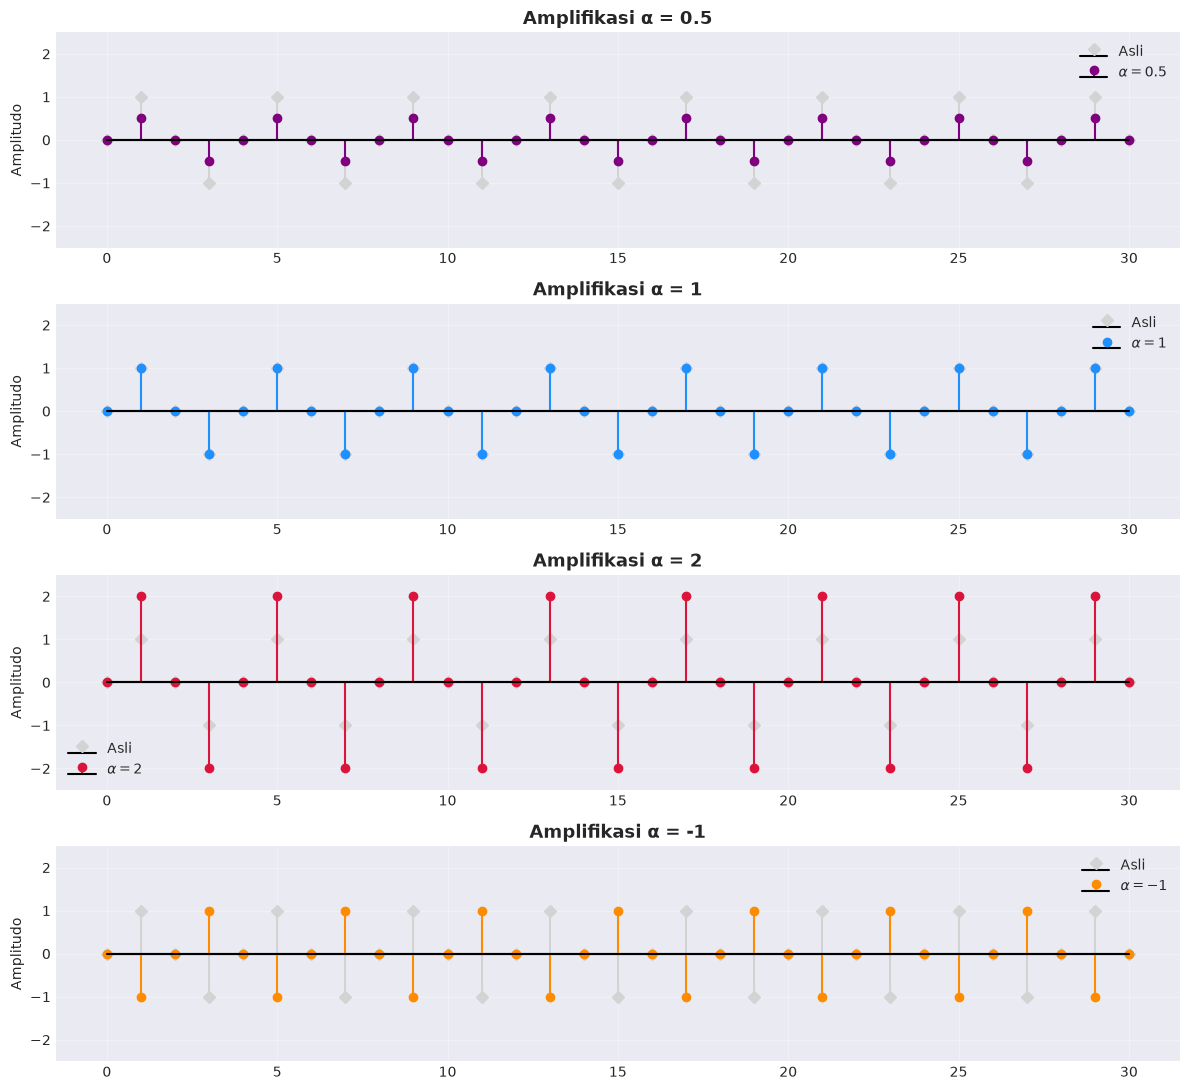
\includegraphics[width=0.55\textwidth]{amplifikasi_sinyal.png}
\caption{Hasil amplifikasi sinyal dengan berbagai nilai $\alpha$.}
\end{figure}

\begin{table}[h]
\centering
\caption{Efek nilai $\alpha$ terhadap sinyal.}
\begin{tabular}{cc}
\toprule
$\alpha$ & Efek \\
\midrule
0.5 & Atenuasi 50\% (volume mengecil) \\
1   & Sinyal asli (gain satuan) \\
2   & Amplifikasi 2$\times$ (volume membesar) \\
-1  & Inversi fasa 180$^\circ$ \\
\bottomrule
\end{tabular}
\end{table}

$\alpha > 1$ memperkuat sinyal namun berisiko \textit{clipping}. $0 < \alpha < 1$ memperlemah sinyal (\textit{volume control}). $\alpha$ negatif membalik fase sinyal, yang menjadi dasar \textit{noise cancellation}.

% ============================================================
\section{Operasi pada Citra 2D}
% ============================================================

\subsection{Membaca dan Menampilkan Citra}

Citra yang digunakan berukuran $300 \times 200$ piksel, tipe data \texttt{uint8}, dengan rentang nilai piksel 52--255.

\subsection{Penjumlahan Citra}

Dua citra dengan ukuran sama dijumlahkan secara element-wise. Jika ukuran berbeda, dilakukan \textit{resizing} terlebih dahulu. Dua metode digunakan:
\begin{itemize}
\item \textbf{Clipping}: hasil $>255$ dipotong ke 255, menyebabkan hilangnya detail pada area terang.
\item \textbf{Normalisasi}: hasil diskalakan ke rentang $[0,255]$, detail terjaga namun kontras berkurang.
\end{itemize}

\begin{figure}[h]
\centering
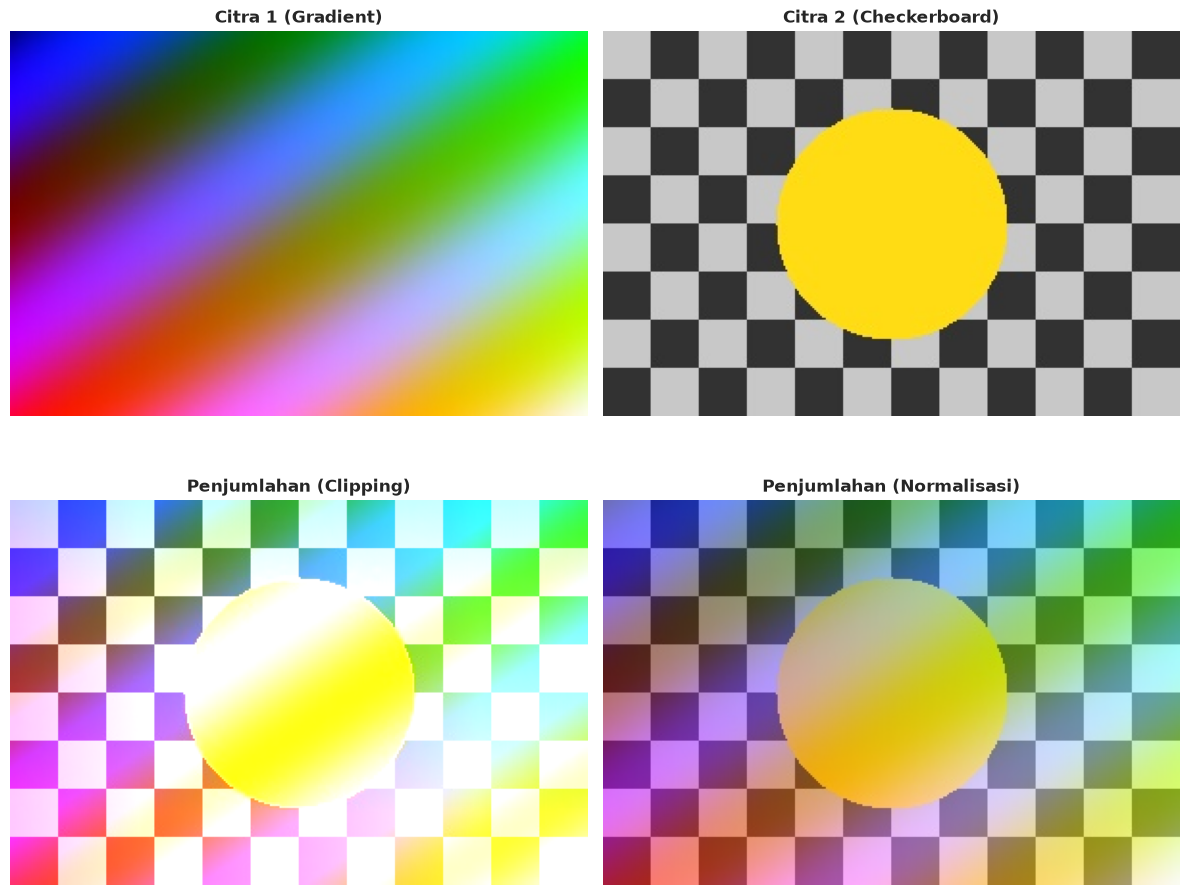
\includegraphics[width=0.65\textwidth]{penjumlahan_citra.png}
\caption{Perbandingan clipping vs normalisasi pada penjumlahan citra.}
\end{figure}

Aplikasi nyata: \textit{image blending}, \textit{long exposure photography}, dan \textit{medical image fusion}.

\subsection{Penggeseran Citra (Translasi)}

Translasi $I'(i,j) = I(i-\Delta i, j-\Delta j)$ diuji dengan tiga kombinasi: vertikal $(\Delta i=30)$, horizontal $(\Delta j=30)$, dan diagonal $(30,30)$.

\begin{figure}[h]
\centering
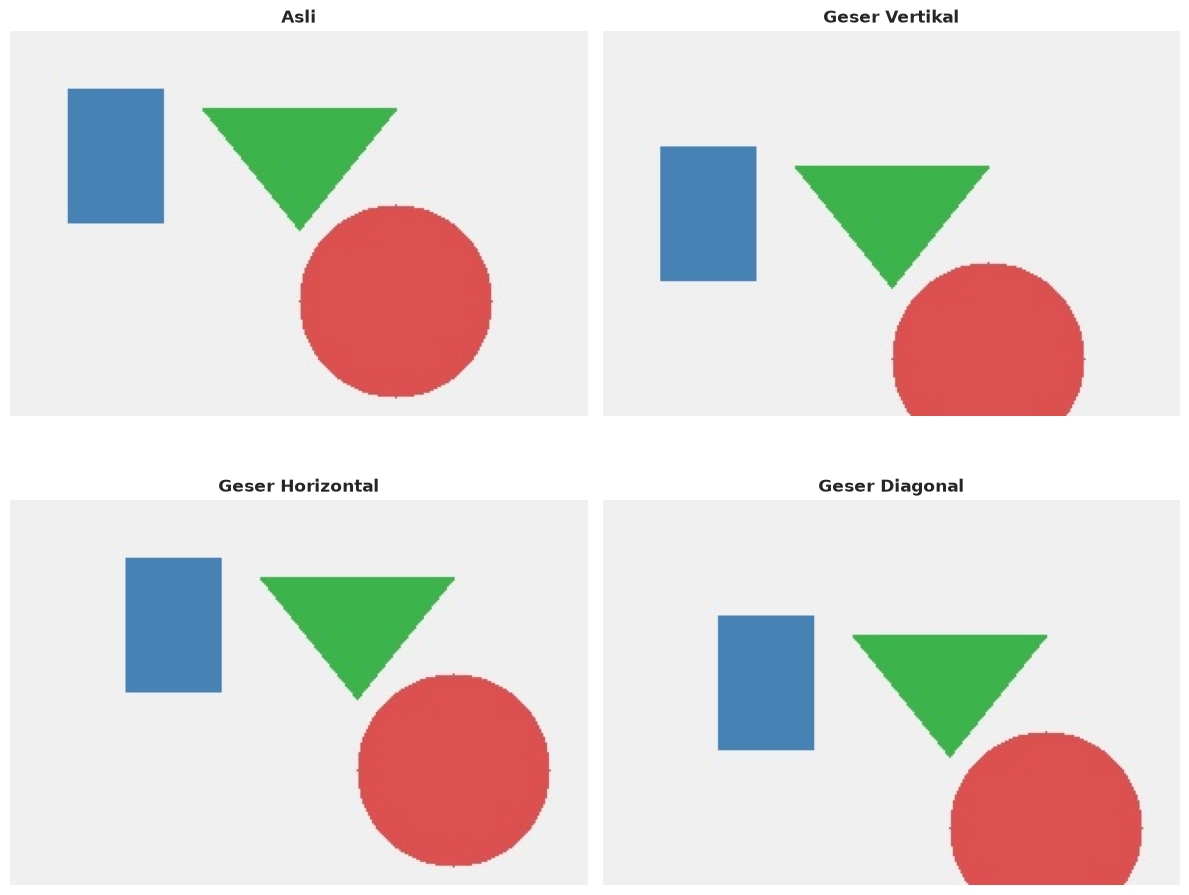
\includegraphics[width=0.6\textwidth]{penggeseran_citra.png}
\caption{Hasil translasi citra dengan berbagai arah.}
\end{figure}

Area kosong yang muncul diisi dengan latar abu-abu (240). Penggeseran dalam augmentasi data membuat model menjadi \textit{shift-invariant}. Risiko: objek bisa keluar \textit{frame} jika pergeseran terlalu besar.

\subsection{Amplifikasi Citra}

Amplifikasi $I'(i,j) = \alpha I(i,j)$ diuji dengan $\alpha = 0.5$, $1.0$, $1.5$, $2.0$.

\begin{figure}[h]
\centering
\begin{subfigure}{0.47\textwidth}
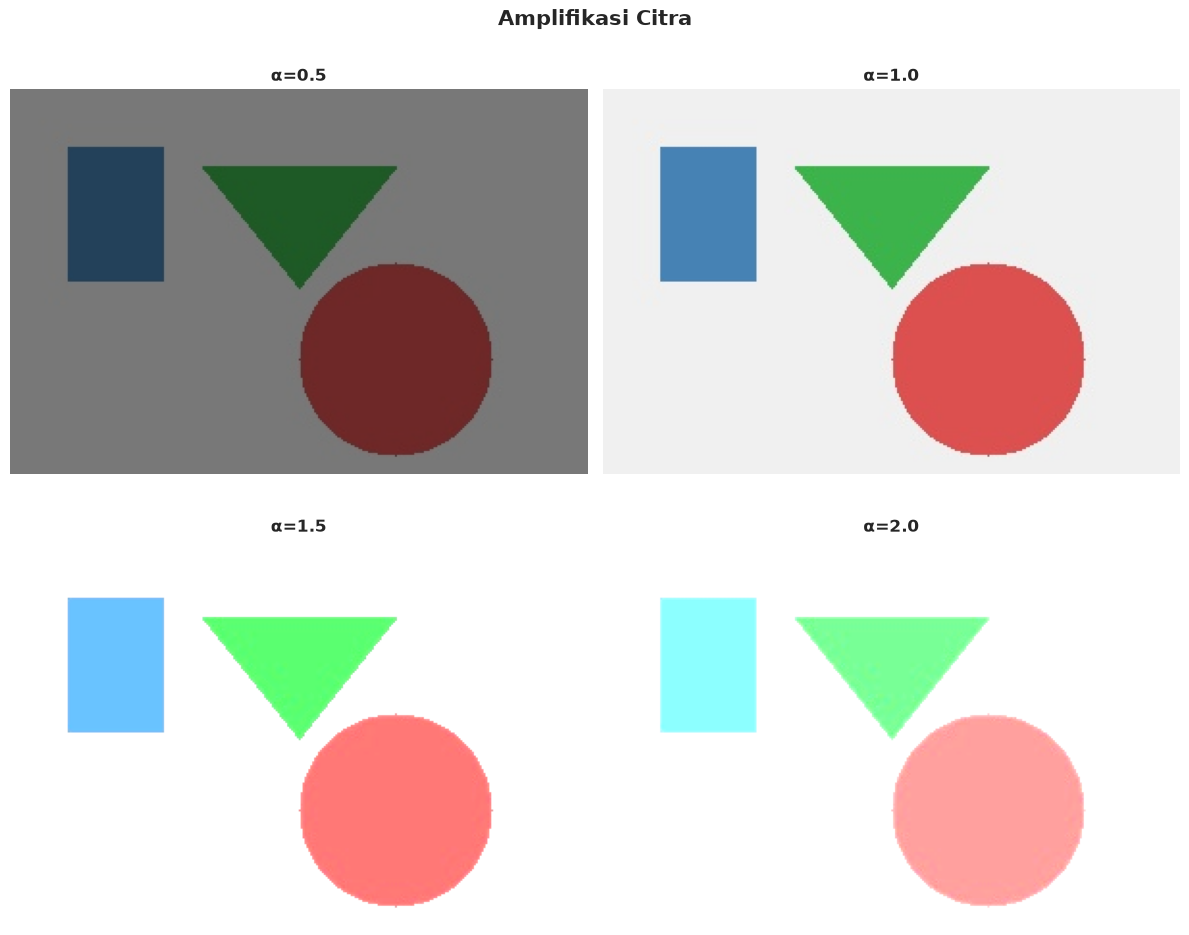
\includegraphics[width=\textwidth]{amplifikasi_citra.png}
\caption{Amplifikasi citra}
\end{subfigure}
\hfill
\begin{subfigure}{0.47\textwidth}
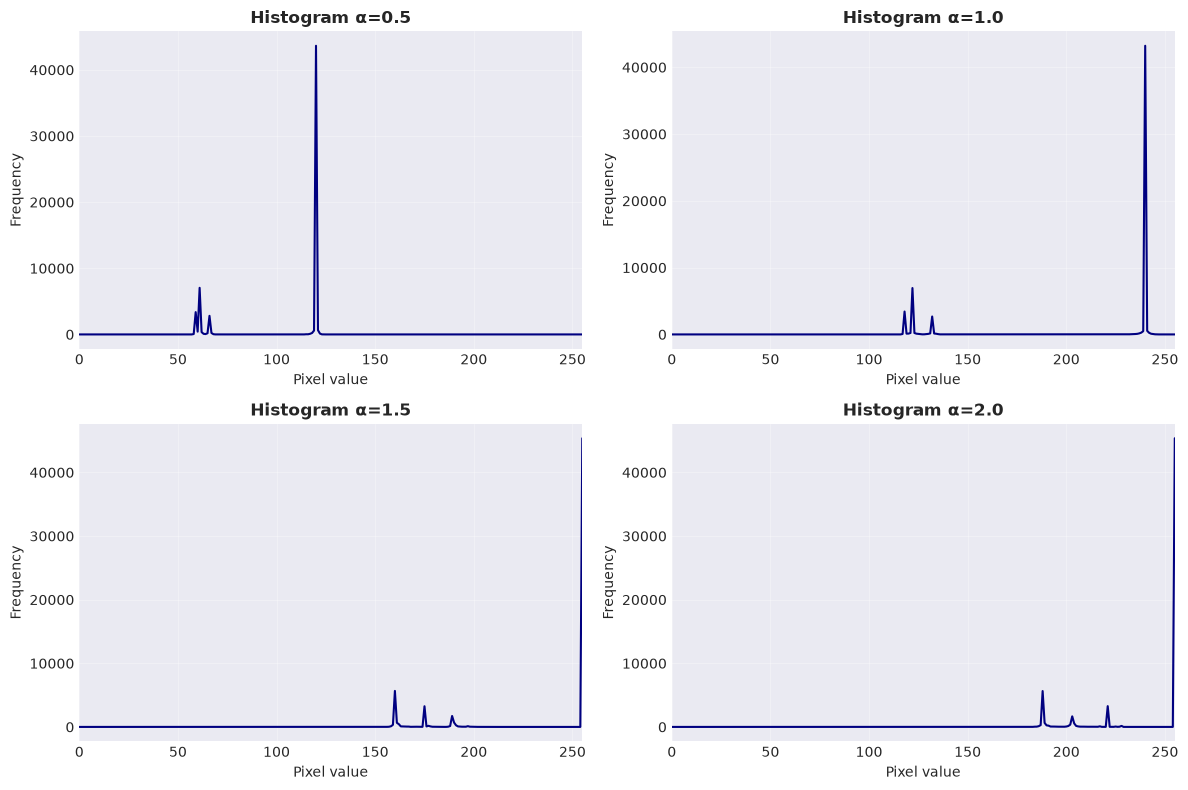
\includegraphics[width=\textwidth]{histogram_amplifikasi.png}
\caption{Histogram}
\end{subfigure}
\caption{Hasil amplifikasi citra dan histogramnya untuk berbagai $\alpha$.}
\end{figure}

$\alpha > 1$ meningkatkan \textit{brightness} dan kontras, tetapi nilai $>255$ akan di-\textit{clip}. $0 < \alpha < 1$ mengurangi \textit{brightness}. Pembatasan nilai piksel penting karena citra \texttt{uint8} hanya memiliki rentang 0--255.

% ============================================================
\section{Uji Sistem Linier}
% ============================================================

Sistem linier harus memenuhi dua sifat: homogenitas $\big(T(\alpha x) = \alpha T(x)\big)$ dan additivitas $\big(T(x_1+x_2) = T(x_1)+T(x_2)\big)$.

\subsection{Uji Homogenitas}

Sistem $T(x)=2x$ diuji dengan $\alpha = 0.5$, $2$, $-1$. Hasil $T(\alpha x)$ dan $\alpha T(x)$ identik untuk semua nilai $\alpha$ (selisih $<10^{-10}$), membuktikan homogenitas.

\subsection{Uji Additivitas}

Dengan $x_1[n] = \sin(0.5\pi n)$ dan $x_2[n] = u[n-5]$, nilai $T(x_1+x_2)$ identik dengan $T(x_1)+T(x_2)$ (selisih $0$), membuktikan additivitas.

\subsection{Perbandingan Linier vs Non-Linier}

\begin{table}[h]
\centering
\caption{Perbandingan sistem linier dan non-linier.}
\begin{tabular}{lccc}
\toprule
Sistem & Homogenitas & Additivitas & Linier? \\
\midrule
$T_1(x)=2x$ & Ya & Ya & \textbf{Linier} \\
$T_2(x)=x^2$ & Tidak & Tidak & \textbf{Non-linier} \\
\bottomrule
\end{tabular}
\end{table}

$T_2(x)=x^2$ gagal pada homogenitas karena $(\alpha x)^2 = \alpha^2 x^2 \neq \alpha \cdot x^2$, dan gagal pada additivitas karena $(x_1+x_2)^2 = x_1^2 + 2x_1x_2 + x_2^2 \neq x_1^2 + x_2^2$. Suku silang $2x_1x_2$ menyebabkan sistem non-linier.

\begin{figure}[h]
\centering
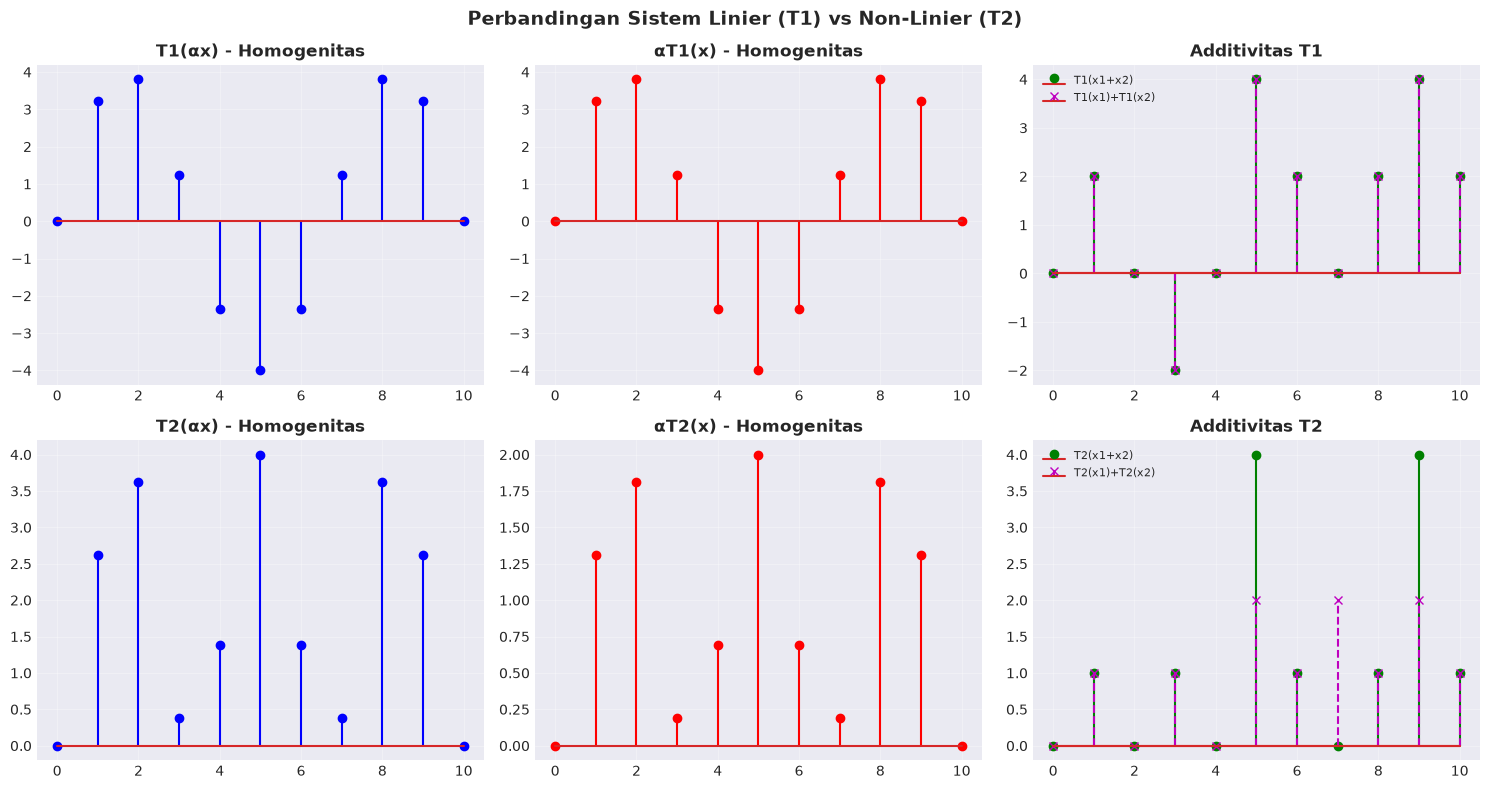
\includegraphics[width=0.7\textwidth]{perbandingan_sistem.png}
\caption{Perbandingan uji homogenitas dan additivitas untuk $T_1$ dan $T_2$.}
\end{figure}

Sistem linier penting karena memungkinkan prinsip superposisi: respons terhadap kombinasi input sama dengan kombinasi respons individual. Ini menjadi dasar analisis Fourier, perancangan filter, dan pemrosesan sinyal modern.

% ============================================================
\section{Analisis HOTS}
% ============================================================

\subsection{Analisis Konseptual}

\textbf{1. Penjumlahan dan amplifikasi sebagai dasar superposisi:} Superposisi adalah kombinasi linier dari sinyal. Kombinasi linier terdiri dari operasi amplifikasi (perkalian dengan skalar) dan penjumlahan. Dengan demikian, sistem yang memenuhi superposisi secara otomatis membutuhkan kedua operasi ini sebagai fondasi.

\textbf{2. Tidak semua operasi linier:} Operasi seperti $x^2$, $\sin(x)$, dan \textit{thresholding} tidak memenuhi homogenitas dan additivitas. Misalnya, mengkuadratkan sinyal menghasilkan harmonik baru yang tidak ada pada sinyal asli.

\textbf{3. Dampak sistem non-linier:} Menghasilkan harmonik baru, distorsi intermodulasi, dan superposisi tidak berlaku. Output tidak dapat diprediksi dari input individual.

\textbf{4. Pentingnya shift dan amplify:} \textit{Shift} adalah dasar dari \textit{delay}, \textit{echo}, dan estimasi gerak. \textit{Amplify} adalah dasar dari \textit{gain}, volume, dan kecerahan. Keduanya adalah blok fundamental DSP.

\subsection{Studi Kasus: Audio Mixing}

\textbf{Masalah:} Mencampur beberapa \textit{track} audio menjadi satu \textit{master track} yang seimbang.

\textbf{Operasi yang digunakan:} Penjumlahan (mencampur sinyal), amplifikasi (\textit{gain control} tiap \textit{track}), dan penggeseran (\textit{delay} untuk efek spasial).

\textbf{Relevansi:} Pencampuran audio adalah contoh langsung superposisi sinyal. Setiap instrumen adalah sinyal terpisah yang dijumlahkan setelah diamplifikasi dengan \textit{gain} tertentu.

\textbf{Linieritas:} Operasi mixing dasar bersifat linier (penjumlahan + gain). Namun, praktik nyata melibatkan kompresor, limiter, dan saturasi yang bersifat non-linier.

\textbf{Kelebihan:} Sederhana, $O(N)$, hasil mudah diprediksi. \textbf{Kekurangan:} Tidak memodelkan saturasi pita magnetik, \textit{noise masking}, dan efek non-linier lainnya.

\subsection{Skenario Pengambilan Keputusan}

\textbf{S1 -- Image blending ukuran berbeda:} Kedua citra harus di-\textit{resize} ke ukuran yang sama karena operasi penjumlahan bersifat \textit{element-wise} dan membutuhkan padanan piksel yang tepat.

\textbf{S2 -- Audio terlalu kecil:} Lakukan amplifikasi dengan $\alpha > 1$. Risiko: \textit{clipping} pada amplitudo puncak yang menyebabkan distorsi.

\textbf{S3 -- Deteksi objek gagal karena variasi posisi:} Gunakan translasi acak sebagai augmentasi data agar model menjadi \textit{shift-invariant} dan mampu mendeteksi objek di berbagai posisi.

\textbf{S4 -- Output berbeda saat urutan filter dan amplifikasi ditukar:} Sistem tersebut kemungkinan non-linier, karena sistem LTI (Linier Time-Invariant) bersifat komutatif terhadap \textit{cascade}.

% ============================================================
\section{Kesimpulan dan Refleksi Pribadi}
% ============================================================

\subsection{Kesimpulan}

Eksperimen ini menunjukkan bahwa operasi sederhana seperti penjumlahan, penggeseran, dan amplifikasi merupakan blok bangunan fundamental dari konsep yang lebih besar dalam Pengolahan Sinyal Digital. Sistem linier, yang memenuhi homogenitas dan additivitas, memungkinkan penggunaan prinsip superposisi untuk analisis sinyal yang kompleks. Pada citra 2D, operasi yang sama menghasilkan efek visual yang berbeda (perubahan brightness, translasi objek, image blending) dengan tantangan tersendiri seperti clipping dan saturasi.

\subsection{Refleksi Pribadi}

\begin{enumerate}
\item \textbf{Operasi termudah:} Amplifikasi, karena hanya perkalian skalar yang intuitif.
\item \textbf{Operasi tersulit:} Penggeseran dengan \textit{zero-padding}, karena perlu menangani batas sinyal dengan benar.
\item \textbf{Perbedaan 1D vs 2D:} Citra memiliki dua dimensi spasial dan tiga \textit{channel} warna, sehingga operasi dilakukan pada matriks 3D.
\item \textbf{Insight baru:} Fungsi sesederhana $x^2$ saja sudah cukup untuk mematahkan sifat linier karena menghasilkan suku silang.
\item \textbf{Bagian paling penting:} Konsep superposisi dan linieritas merupakan dasar dari filtering, kompresi, dan analisis spektrum dalam DSP.
\end{enumerate}

\end{document}
